%%%%%%%%%%%%%%%%%%%%%%%%%%%%%%%%%%%%%%%%%%%%%%%%%%%%%%%%%%%%%%%%%%%%%%%%%%%%%%%%
% Zynq Platform
%%%%%%%%%%%%%%%%%%%%%%%%%%%%%%%%%%%%%%%%%%%%%%%%%%%%%%%%%%%%%%%%%%%%%%%%%%%%%%%%
\subsection{Zynq Platform}
\begin{frame}[label=zynq]{Zynq Platform}
    \makebox[\textwidth][c]{
        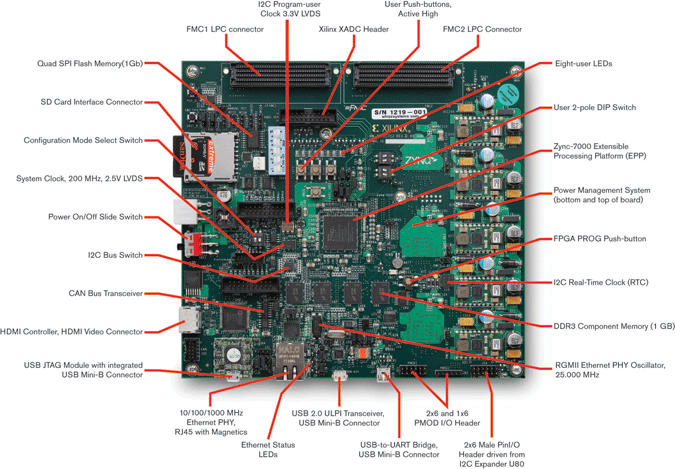
\includegraphics[height=0.88\textheight]{xilinx/zc702-base-board}}
\end{frame}

%%%%%%%%%%%%%%%%%%%%%%%%%%%%%%%%%%%%%%%%%%%%%%%%%%%%%%%%%%%%%%%%%%%%%%%%%%%%%%%%
% Design
%%%%%%%%%%%%%%%%%%%%%%%%%%%%%%%%%%%%%%%%%%%%%%%%%%%%%%%%%%%%%%%%%%%%%%%%%%%%%%%%
% In this section, illustrate the hardware and software interface for the
% design. Note that the most important part of the hardware design is
% parallelism, so it is important to mention how this was achieved.
\subsection{Design}
\begin{frame}[label=design]{Design}
    % Block diagram showing hardware, software and interface
    % Multiple functional units
    % Instruction level parallelism
    % Pipelining
\end{frame}

%%%%%%%%%%%%%%%%%%%%%%%%%%%%%%%%%%%%%%%%%%%%%%%%%%%%%%%%%%%%%%%%%%%%%%%%%%%%%%%%
% Results
%%%%%%%%%%%%%%%%%%%%%%%%%%%%%%%%%%%%%%%%%%%%%%%%%%%%%%%%%%%%%%%%%%%%%%%%%%%%%%%%
\subsection{Results}
% How many cycles the hardware design takes
% Reference to Amdahl's Law
% "On this hardware, we expect a speed up of X"
% Performance estimates
% Performance comparison
% Complexity (scaling)
\begin{frame}[label=performance-considerations]{Performance Considerations}
    \begin{itemize}
        \item Cannot be data transfer faster than $O(n)$
        \item For each vector that is pruned from the block, we save (on
            average) $\frac{block\_size}{2}$ distance computations
    \end{itemize}
\end{frame}

\begin{frame}[label=performance-estimates]{Performance Estimates}
    The execution time for the proposed design is estimated to be the sum of:
    \begin{enumerate}
        \item<1-> Execution time of software implementation, excluding the
            distance\_squared function
        \item<2-> Time required for DMA transfer of ``outer'' vector.
        \item<3-> Time required for DMA transfer of ``inner'' vector, plus the time
            required for the hardware to complete the computation and return the
            result
        \item<4-> Overheads associated with thread management
    \end{enumerate}
\end{frame}
